\documentclass[12pt,french,oneside]{report}
%%%%%%%%%%%%%%%%%%%%%%%%%%%%%%%%%%%%%%%%%%%%%%%%%%%%%%%%%%%%%%%%%%%%%%%%%%%%%%%
\input{preambule_2017}
%\input{preambule_2015}
%%___________________________
%===   Redéfinition des marges par défaut
%------------------------------------------------------
%\usepackage[textwidth=18.6cm]{geometry}%à mettre dans le preambule perso
%\pagestyle{fancy}%à mettre dans le preambule perso


\setlength\paperheight{297mm}
\setlength\paperwidth{210mm}
\setlength{\evensidemargin}{0cm}% Marge gauche sur pages paires
\setlength{\oddsidemargin}%{0cm}%
{-0.5cm}% Marge gauche sur pages impaires
\setlength{\topmargin}{-2cm}% Marge en haut
\setlength{\headsep}{0.5cm}% Entre le haut de page et le texte
\setlength{\headheight}{0.7cm}% Haut de page
\setlength{\textheight}{25.2cm}% Hauteur de la zone de texte
\setlength{\textwidth}{17cm}% Largeur de la zone de texte


% Environnement enumerate
\renewcommand{\theenumi}{\bf\textsf{\arabic{enumi}}}
\renewcommand{\labelenumi}{\bf\textsf{\theenumi.}}
\renewcommand{\theenumii}{\bf\textsf{\alph{enumii}}}
\renewcommand{\labelenumii}{\bf\textsf{\theenumii.}}
\renewcommand{\theenumiii}{\bf\textsf{\roman{enumiii}}}
\renewcommand{\labelenumiii}{\bf\textsf{\theenumiii.}}


\usetikzlibrary{shadows,trees}


%definition des couleurs
\definecolor{fondpaille}{cmyk}{0,0,0.1,0}%\pagecolor{fondpaille}
\definecolor{gris}{rgb}{0.7,0.7,0.7}
\definecolor{rouge}{rgb}{1,0,0}
\definecolor{bleu}{rgb}{0,0,1}
\definecolor{vert}{rgb}{0,1,0}
\definecolor{deficolor}{HTML}{2D9AFF}
\definecolor{backdeficolor}{HTML}{EDEDED}%{036DD0}%dégradé bleu{666666}%dégradé gris
\definecolor{theocolor}{HTML}{036DD0}%F4404D%rouge
\definecolor{backtheocolor}{HTML}{D3D3D3}
\definecolor{methcolor}{HTML}{008800}%12BB05}
\definecolor{backmethcolor}{HTML}{FFFACD}
\definecolor{backilluscolor}{HTML}{EDEDED}
\definecolor{sectioncolor}{HTML}{221E1E}%{B2B2B2}%vert : {HTML}{008800}%{HTML}{2D9AFF}
\definecolor{subsectioncolor}{HTML}{221E1E}%{B2B2B2}%vert : {HTML}{008800}%{rgb}{0.5,0,0}
\definecolor{engcolor}{HTML}{D4D7FE}
\definecolor{exocolor}{rgb}{0,0.6,0}
\definecolor{exosoltitlecolor}{rgb}{0,0.6,0}
\definecolor{titlecolor}{rgb}{1,1,1}

%commande pour enlever les couleurs avant impression
\newcommand{\nocolor}
{\pagecolor{white}
\definecolor{gris}{rgb}{0.7,0.7,0.7}
\definecolor{rouge}{rgb}{0,0,0}
\definecolor{bleu}{rgb}{0,0,0}
\definecolor{vert}{rgb}{0,0,0}
\definecolor{deficolor}{HTML}{B2B2B2}
\definecolor{backdeficolor}{HTML}{EEEEEE}%{036DD0}%dégradé bleu{666666}%dégradé gris
\definecolor{theocolor}{HTML}{B2B2B2}
\definecolor{backtheocolor}{HTML}{EEEEEE}
\definecolor{methcolor}{HTML}{B2B2B2}
\definecolor{backmethcolor}{HTML}{EEEEEE}
\definecolor{backilluscolor}{HTML}{EEEEEE}
\definecolor{sectioncolor}{HTML}{B2B2B2}
\definecolor{subsectioncolor}{HTML}{B2B2B2}
\definecolor{engcolor}{HTML}{EEEEEE}
\definecolor{exocolor}{HTML}{3B3838}
\definecolor{exosoltitlecolor}{rgb}{0,0,0}
\definecolor{titlecolor}{rgb}{0,0,0}
}



%___________________________
%===    Exercice résolu
%------------------------------------------------------
%
%#1 : énoncé
%#2 : solution
\newcounter{exosol}
\newcommand{\exosol}[2]{
\stepcounter{exosol}
\begin{tikzpicture}[node distance=0 cm]
\node[fill=backilluscolor,rounded corners=2pt,anchor=south west] (illus) at (0,-0.02)
{\it \textbf{\textcolor{exosoltitlecolor}{Exercice résolu \arabic{exosol}~:~}}};
\node[fill=backilluscolor,rounded corners=2pt,anchor=north west]at(0,0)
{\parbox{\columnwidth-10pt}{#1\par\medskip{\it \textbf{\textcolor{exosoltitlecolor}{Solution~:~}}}\par#2 }};
\end{tikzpicture}
\bigskip
}

\newcommand{\suite}[1]{
\begin{tikzpicture}[node distance=0 cm]
\node[fill=backilluscolor,rounded corners=2pt,anchor=north west]at(0,0)
{\parbox{\columnwidth-10pt}{{\it \textbf{\textcolor{exosoltitlecolor}{Suite de la solution~:}}}\par#1}};
\end{tikzpicture}
\bigskip
}



%%%%%%%%%%%%%%%%%%%%%%%%%%%%%%%%%%%%%%%%%%%%%%%%%%%%%%%%%%%%%%%%%%%%%%%%%%%%%%%
%Encadrés pour Propriétés, Théorème, Définitions, exemples, exercices

\usepackage{environ}%pour pouvoir utiliser la commande \NewEnviron

%___________________________
%===    Propriété avec ou sans s et avec ou sans titre
%------------------------------------------------------
%
\NewEnviron{Prop}[2][]{
\begin{tikzpicture}[node distance=0 cm]
\node[fill=theocolor,rounded corners=5pt,anchor=south west] (theorem) at (0,0)
{\textcolor{titlecolor}{Propriété#1~:~#2}};
\node[draw,drop shadow,color=theocolor,very thick,fill=backtheocolor,rounded corners=5pt,anchor=north west] at(0,-0.02)
{\black\parbox{\columnwidth-12pt}{\BODY}};
\end{tikzpicture}
\bigskip
}


%___________________________
%===    Conséquence avec ou sans s et avec ou sans titre
%------------------------------------------------------
%
\NewEnviron{Cons}[2][]{
\begin{tikzpicture}[node distance=0 cm]
\node[fill=theocolor,rounded corners=5pt,anchor=south west] (theorem) at (0,0)
{\textcolor{titlecolor}{Conséquence#1~:~#2}};
\node[draw,drop shadow,color=theocolor,very thick,fill=backtheocolor,rounded corners=5pt,anchor=north west] at(0,-0.02)
{\black\parbox{\columnwidth-12pt}{\BODY}};
\end{tikzpicture}
\bigskip
}


%___________________________
%===    Théorème avec ou sans titre
%------------------------------------------------------
%
\NewEnviron{Thm}[1][]{
\begin{tikzpicture}[node distance=0 cm]
\node[fill=theocolor,rounded corners=5pt,anchor=south west] (theorem) at (0,0)
{\textcolor{titlecolor}{Théorème~:~#1}};
\node[draw,drop shadow,color=theocolor,very thick,fill=backtheocolor,rounded corners=5pt,anchor=north west] at(0,-0.02)
{\black\parbox{\columnwidth-12pt}{\BODY}};
\end{tikzpicture}
\medskip
}


%___________________________
%===    Cadre arrondi coloré
%------------------------------------------------------
%
\NewEnviron{CadreColor}{

\begin{tikzpicture}[node distance=0 cm]
\node[draw,drop shadow,color=theocolor,very thick,fill=backtheocolor,rounded corners=5pt,anchor=north west] at(0,-0.02)
{\black\parbox{\columnwidth-12pt}{\BODY}};
\end{tikzpicture}
\medskip
}


%___________________________
%===    Cadre arrondi blanc
%------------------------------------------------------
%
\NewEnviron{Cadre}{
\begin{tikzpicture}[node distance=0 cm]
\node[draw,very thick,rounded corners=5pt,anchor=north west] at(0,-0.02)
{\black\parbox{\columnwidth-12pt}{\BODY}};
\end{tikzpicture}
\medskip
}



%___________________________
%===    Règle(s) avec ou sans s et avec sans titre
%------------------------------------------------------
%
\NewEnviron{Regle}[2][]{
\begin{tikzpicture}[node distance=0 cm]
\node[fill=theocolor,rounded corners=5pt,anchor=south west] (theorem) at (0,0)
{\textcolor{titlecolor}{Règle#1~:~#2}};
\node[draw,drop shadow,color=deficolor,very thick,fill=backdeficolor,rounded corners=5pt,anchor=north west] at(0,-0.02)
{\black\parbox{\columnwidth-12pt}{\BODY}};
\end{tikzpicture}
\medskip
}

%___________________________
%===    Définition avec ou sans s et avec sans titre
%------------------------------------------------------
%
\NewEnviron{Defi}[2][]{
\begin{tikzpicture}[node distance=0 cm]
\node[fill=theocolor,rounded corners=5pt,anchor=south west] (theorem) at (0,0)
{\textcolor{titlecolor}{Définition#1~:~#2}};
\node[draw,drop shadow,color=deficolor,very thick,fill=backdeficolor,rounded corners=5pt,anchor=north west] at(0,-0.02)
{\black\parbox{\columnwidth-12pt}{\BODY}};
\end{tikzpicture}
\medskip
}

%___________________________
%===    Méthode avec ou sans s et avec sans titre
%------------------------------------------------------
%
\NewEnviron{Methode}[2][]{
\begin{tikzpicture}[node distance=0 cm]
\node[fill=theocolor,rounded corners=5pt,anchor=south west] (theorem) at (0,0)
{\textcolor{titlecolor}{Méthode#1~:~#2}};
\node[draw,drop shadow,color=methcolor,very thick,fill=backmethcolor,rounded corners=5pt,anchor=north west] at(0,-0.02)
{\black\parbox{\columnwidth-12pt}{\BODY}};
\end{tikzpicture}
\medskip
}


%___________________________
%===    Redéfinition de la commande \chapter{•}
%------------------------------------------------------
%
\makeatletter

\renewcommand{\@makechapterhead}[1]{
\begin{tikzpicture}
\node[fill=theocolor,rectangle,rounded corners=5pt]{%
\begin{minipage}{\linewidth}
\begin{center}
\vspace*{9pt}
\textcolor{titlecolor}{\Large \textsc{\textbf{Chapitre \thechapter \ : \ #1}}}
\vspace*{9pt}
\end{center}
\end{minipage}
};\end{tikzpicture}
}

\makeatother


%___________________________
%===    Exemple avec ou sans s et avec ou sans titre
%------------------------------------------------------
%
\NewEnviron{Exemple}[2][]{
\begin{tikzpicture}[node distance=0 cm]
\node[draw,drop shadow,color=methcolor,very thick,fill=backmethcolor,rounded corners=5pt,anchor=north west] at(0,-0.02)
{\black\parbox{\columnwidth-12pt}{\textbf{Exemple#1~:~#2}\\
\BODY}};
\end{tikzpicture}
\medskip
}

%___________________________
%===    Remarque avec ou sans s
%------------------------------------------------------
%
\NewEnviron{Rmq}[1][]{
\textbf{\large{Remarque#1 :}}\par
\BODY
\medskip
}

%___________________________
%===    Remarques numérotées R1, R2, etc...
%------------------------------------------------------
%
\newcounter{rem}\newcommand{\rem}{\refstepcounter{rem}\textbf{R \therem \ :}\xspace}

%___________________________
%===    Exercices du contrôle numérotés
%------------------------------------------------------
%
\newcounter{exercice}
\NewEnviron{Exercice}[1][]{
\refstepcounter{exercice}\textbf{\large{Exercice \theexercice \ :}}\hfill \textbf{#1}\par
\BODY
\medskip
}

%___________________________
%===    Exercices non numérotés
%------------------------------------------------------
%
\NewEnviron{Exo}[1][]{
\textbf{\large{Exercice #1 \ :}}\par
\BODY
\medskip
}

%___________________________
%===    Démonstration
%------------------------------------------------------
\NewEnviron{Demo}{%
\textit{\textbf{Démonstration.}}\par
\BODY
\strut\hfill$\square$
\medskip
}

%___________________________
%===    Commandes perso
%------------------------------------------------------
%
%\Leftrightarrow
\newcommand{\Lr}{\Leftrightarrow}

%Ancienne commande chapitre
\newcommand{\chapitre}[1]{
\begin{tikzpicture}
\node[fill=theocolor,rectangle,rounded corners=5pt]{%
\begin{minipage}{\linewidth}
\begin{center}
\vspace*{9pt}
\textcolor{titlecolor}{\Large \textsc{\textbf{#1}}}
\vspace*{9pt}
\end{center}
\end{minipage}
};
\end{tikzpicture}
\bigskip
}

%Pour les fiches : commande de Cécile
\newcommand{\Fiche}[2]{%
\begin{tikzpicture}
	\node[draw, color=blue,fill=white,rectangle,rounded corners=5pt]{%
	\begin{minipage}{\linewidth}
		\begin{center}
			\vspace*{9pt}
			\textcolor{blue}{\Large \textsc{\textbf{Fiche~#1\ :\ #2}}}
			\vspace*{7pt}
		\end{center}
	\end{minipage}
	};
\end{tikzpicture}
}%

\pagecolor{white}%couleur du fond de page

\renewcommand{\Pointilles}{%
\makebox[\linewidth]{\dotfill}
}


%centrer du texte ou une formule avec moins d'espace autour
\newcommand{\centrer}[1]
{
\smallskip
\centerline{#1}
\smallskip
}


%QRcode généré par le package qrcode
\usepackage{qrcode}


%Pour pouvoir utiliser l'environnement verbatim
\usepackage{verbatim}

%Panneau danger (nécessite le package pstricks)
\def\danger{\begingroup
\psset{unit=1ex}%
\begin{pspicture}(0,0)(3,3)
 
\pspolygon[linearc=0.2,linewidth=0.12,linecolor=red](0,0)(1.5,2.6)(3,0)
 
\psellipse*(1.5,1.33)(0.14,0.75)\pscircle*(1.5,0.3){0.15}\end{pspicture}
%
\endgroup}%

%___________________________
%===    Nouvelles commandes pour documents venant de Sesamath
%------------------------------------------------------
%
\definecolor{CyanTikz40}{cmyk}{.4,0,0,0}
\definecolor{CyanTikz20}{cmyk}{.2,0,0,0}
\tikzstyle{general}=[line width=0.3mm, >=stealth, x=1cm, y=1cm,line cap=round, line join=round]
\tikzstyle{quadrillage}=[line width=0.3mm, color=CyanTikz40]
\tikzstyle{quadrillageNIV2}=[line width=0.3mm, color=CyanTikz20]
\tikzstyle{quadrillage55}=[line width=0.3mm, color=CyanTikz40, xstep=0.5, ystep=0.5]
\tikzstyle{cote}=[line width=0.3mm, <->]
\tikzstyle{epais}=[line width=0.5mm, line cap=butt]
\tikzstyle{tres epais}=[line width=0.8mm, line cap=butt]
\tikzstyle{axe}=[line width=0.3mm, ->, color=Noir, line cap=rect]
\newcommand{\quadrillageSeyes}[2]{\draw[line width=0.3mm, color=A1!10, ystep=0.2, xstep=0.8] #1 grid #2;
\draw[line width=0.3mm, color=A1!30, xstep=0.8, ystep=0.8] #1 grid #2; }
\newcommand{\axeX}[4][0]{\draw[axe] (#2,#1)--(#3,#1); \foreach \x in {#4} {\draw (\x,#1) node {\small $+$}; \draw (\x,#1) node[below] {\small $\x$};}}
\newcommand{\axeY}[4][0]{\draw[axe] (#1,#2)--(#1,#3); \foreach \y in {#4} {\draw (#1, \y) node {\small $+$}; \draw (#1, \y) node[left] {\small $\y$};}}
\newcommand{\axeOI}[3][0]{\draw[axe] (#2,#1)--(#3,#1);  \draw (1,#1) node {\small $+$}; \draw (1,#1) node[below] {\small $I$};}
\newcommand{\axeOJ}[3][0]{\draw[axe] (#1,#2)--(#1,#3); \draw (#1, 1) node {\small $+$}; \draw (#1, 1) node[left] {\small $J$};}
\newcommand{\axeXgraduation}[2][0]{\foreach \x in {#2} {\draw (\x,#1) node {\small $+$};}}
\newcommand{\axeYgraduation}[2][0]{\foreach \y in {#2} {\draw (#1, \y) node {\small $+$}; }}
\newcommand{\origine}{\draw (0,0) node[below left] {\small $0$};}
\newcommand{\origineO}{\draw (0,0) node[below left] {$O$};}
\newcommand{\point}[4]{\draw (#1,#2) node[#4] {$#3$};}
\newcommand{\pointGraphique}[4]{\draw (#1,#2) node[#4] {$#3$};
\draw (#1,#2) node {$+$};}
\newcommand{\pointFigure}[4]{\draw (#1,#2) node[#4] {$#3$};
\draw (#1,#2) node {$\times$};}
\newcommand{\pointC}[3]{\draw (#1) node[#3] {$#2$};}
\newcommand{\pointCGraphique}[3]{\draw (#1) node[#3] {$#2$};
\draw (#1) node {$+$};}
\newcommand{\pointCFigure}[3]{\draw (#1) node[#3] {$#2$};
\draw (#1) node {$\times$};}


\definecolor{B1prime}                {cmyk}{0.00, 1.00, 0.00, 0.50}
\definecolor{H1prime}                {cmyk}{0.50, 0.00, 1.00, 0.00}

\definecolor{FootFonctionColor}{cmyk}{0.50, 0.00, 0.00, 0.00}
\definecolor{FootGeometrieColor}{cmyk}{0.40, 0.40, 0.00, 0.00}
\definecolor{FootStatistiqueColor}{cmyk}{0.30, 0.48, 0.00, 0.10}
\definecolor{FootStatistiqueOLDColor}{cmyk}{0.48, 0.30, 0.10, 0.00}
\definecolor{FootStatistique*Color}{cmyk}{0.20, 0.00, 0.00, 0.00}
\definecolor{ActiviteFootColor}{cmyk}{0.50, 0.00, 0.25, 0.00}
\definecolor{CoursFootColor}{cmyk}{0.15, 0.00, 0.00, 0.03}
\definecolor{ExoBaseFootColor}{cmyk}{0.00, 0.25, 0.50, 0.00}
\definecolor{ExoApprFootColor}{cmyk}{0.00, 0.25, 0.50, 0.00}
%\colorlet{ConnFootColor}{F2}
\definecolor{TPFootColor}{cmyk}{0.00, 0.30, 0.00, 0.10}
\definecolor{RecreationFootColor}{cmyk}{0.20, 0.00, 0.50, 0.05}

\definecolor{Blanc}             {cmyk}{0.00, 0.00, 0.00, 0.00}
\definecolor{Gris1}             {cmyk}{0.00, 0.00, 0.00, 0.20}
\definecolor{Gris2}             {cmyk}{0.00, 0.00, 0.00, 0.40}
\definecolor{Gris3}             {cmyk}{0.00, 0.00, 0.00, 0.50}
\definecolor{Noir}              {cmyk}{0.00, 0.00, 0.00, 1.00}
\definecolor{A1}              {cmyk}{0.33, 1.00, 0.00, 0.40}
\definecolor{F1}              {cmyk}{0.00, 1.00, 1.00, 0.00}
\definecolor{C1}              {cmyk}{0.00, 1.00, 0.00, 0.50}
\definecolor{G1}              {cmyk}{0.00, 0.00, 0.00, 0.20}
\definecolor{D1}              {cmyk}{0.00, 0.22, 0.49, 0.69}%bitume
\definecolor{J1}              {cmyk}{0.00, 0.34, 1.00, 0.02}%orangé


%augmenter l'espace au-dessus ou en-dessous d'une fraction
\usepackage{fixltx2e}
\makeatletter
\newcommand*\Strut[1][1]{%
  \leavevmode
  \vrule \@height #1\ht\strutbox
         \@depth #1\dp\strutbox
         \@width\z@
}
\newcommand*\TopStrut[1][1]{%
  \leavevmode
  \vrule \@height #1\ht\strutbox
         \@depth \z@
         \@width \z@
}
\newcommand*\BotStrut[1][1]{%
  \leavevmode
  \vrule \@height \z@
         \@depth #1\dp\strutbox
         \@width \z@
}
\makeatother


% coordonnées vecteurs dans le plan
%\newcommand{\covec2}[2]{\begin{pmatrix}#1\\#2\end{pmatrix}}


% coordonnées dans l'espace
%\newcommand{\covec3}[3]{\begin{pmatrix}#1\\#2\\#3\end{pmatrix}}

% QCM



%%%%%%%%%%%%%%%%%%%%%%%%%%%%%%%%%%%%%%%%%%%%%%%%%%%%%%%%%%%%%%%%%%%%%%%%%%%%%%%
%\input{section_dom_2015_2016}
%%%%%%%%%%%%%%%%%%%%%%%%%%%%%%%%%%%%%%%%%%%%%%%%%%%%%%%%%%%%%%%%%%%%%%%%%%%%%%%

%entête classique

\fancypagestyle{garde_tete}{% 
%\fancyhead[C]{\small\textbf{\seconde} \hfill \small \textbf{Année 2014-2015}}
\renewcommand{\headrulewidth}{0cm}}

\newcommand{\tete}{
\thispagestyle{garde_tete}
\chapitre{Autres exemples TikZ}

\noindent 
\vspace{-6pt}
}

%%%%%%%%%%%%%%%%%%%%%%%%%%%%%%%%%%%%%%%%%%%%%%%%%%%%%%%%%%%%%%%%%%%%%%%%%%%%%%%
%%%%%%%% pour les figures en tikz

%\usepackage{tikz}
%\usepackage{tkz-tab}
%\usepackage{pgf}
%\usetikzlibrary{arrows}
%\usetikzlibrary{patterns}  
\definecolor{CyanTikz40}{cmyk}{.4,0,0,0}
\definecolor{CyanTikz20}{cmyk}{.2,0,0,0}
\tikzstyle{general}=[line width=0.3mm, >=stealth, x=1cm, y=1cm,line cap=round, line join=round]
\tikzstyle{quadrillage}=[line width=0.3mm, color=CyanTikz40]
\tikzstyle{quadrillageNIV2}=[line width=0.3mm, color=CyanTikz20]
\tikzstyle{quadrillage55}=[line width=0.3mm, color=CyanTikz40, xstep=0.5, ystep=0.5]
\tikzstyle{cote}=[line width=0.3mm, <->]
\tikzstyle{epais}=[line width=0.5mm, line cap=butt]
\tikzstyle{tres epais}=[line width=0.8mm, line cap=butt]
\tikzstyle{axe}=[line width=0.3mm, ->, color=Noir, line cap=rect]
%\newcommand{\quadrillageSeyes}[2]{\draw[line width=0.3mm, color=A1!10, ystep=0.2, xstep=0.8] #1 grid #2;
%\draw[line width=0.3mm, color=A1!30, xstep=0.8, ystep=0.8] #1 grid #2; }
%\newcommand{\axeX}[4][0]{\draw[axe] (#2,#1)--(#3,#1); \foreach \x in {#4} {\draw (\x,#1) node {\small $+$}; \draw (\x,#1) node[below] {\small $\x$};}}
%\newcommand{\axeY}[4][0]{\draw[axe] (#1,#2)--(#1,#3); \foreach \y in {#4} {\draw (#1, \y) node {\small $+$}; \draw (#1, \y) node[left] {\small $\y$};}}
%\newcommand{\axeOI}[3][0]{\draw[axe] (#2,#1)--(#3,#1);  \draw (1,#1) node {\small $+$}; \draw (1,#1) node[below] {\small $I$};}
%\newcommand{\axeOJ}[3][0]{\draw[axe] (#1,#2)--(#1,#3); \draw (#1, 1) node {\small $+$}; \draw (#1, 1) node[left] {\small $J$};}
%\newcommand{\axeXgraduation}[2][0]{\foreach \x in {#2} {\draw (\x,#1) node {\small $+$};}}
%\newcommand{\axeYgraduation}[2][0]{\foreach \y in {#2} {\draw (#1, \y) node {\small $+$}; }}
%\newcommand{\origine}{\draw (0,0) node[below left] {\small $0$};}
%\newcommand{\origineO}{\draw (0,0) node[below left] {$O$};}
%\newcommand{\point}[4]{\draw (#1,#2) node[#4] {$#3$};}
%\newcommand{\pointGraphique}[4]{\draw (#1,#2) node[#4] {$#3$};
%\draw (#1,#2) node {$+$};}
%\newcommand{\pointFigure}[4]{\draw (#1,#2) node[#4] {$#3$};
%\draw (#1,#2) node {$\times$};}
%\newcommand{\pointC}[3]{\draw (#1) node[#3] {$#2$};}
%\newcommand{\pointCGraphique}[3]{\draw (#1) node[#3] {$#2$};
%\draw (#1) node {$+$};}
%\newcommand{\pointCFigure}[3]{\draw (#1) node[#3] {$#2$};
%\draw (#1) node {$\times$};}


\definecolor{B1prime}                {cmyk}{0.00, 1.00, 0.00, 0.50}
\definecolor{H1prime}                {cmyk}{0.50, 0.00, 1.00, 0.00}

\definecolor{FootFonctionColor}{cmyk}{0.50, 0.00, 0.00, 0.00}
\definecolor{FootGeometrieColor}{cmyk}{0.40, 0.40, 0.00, 0.00}
\definecolor{FootStatistiqueColor}{cmyk}{0.30, 0.48, 0.00, 0.10}
\definecolor{FootStatistiqueOLDColor}{cmyk}{0.48, 0.30, 0.10, 0.00}
\definecolor{FootStatistique*Color}{cmyk}{0.20, 0.00, 0.00, 0.00}
\definecolor{ActiviteFootColor}{cmyk}{0.50, 0.00, 0.25, 0.00}
\definecolor{CoursFootColor}{cmyk}{0.15, 0.00, 0.00, 0.03}
\definecolor{ExoBaseFootColor}{cmyk}{0.00, 0.25, 0.50, 0.00}
\definecolor{ExoApprFootColor}{cmyk}{0.00, 0.25, 0.50, 0.00}
%\colorlet{ConnFootColor}{F2}
\definecolor{TPFootColor}{cmyk}{0.00, 0.30, 0.00, 0.10}
\definecolor{RecreationFootColor}{cmyk}{0.20, 0.00, 0.50, 0.05}

\definecolor{Blanc}             {cmyk}{0.00, 0.00, 0.00, 0.00}
\definecolor{Gris1}             {cmyk}{0.00, 0.00, 0.00, 0.20}
\definecolor{Gris2}             {cmyk}{0.00, 0.00, 0.00, 0.40}
\definecolor{Gris3}             {cmyk}{0.00, 0.00, 0.00, 0.50}
\definecolor{Noir}              {cmyk}{0.00, 0.00, 0.00, 1.00}
\definecolor{A1}              {cmyk}{0.33, 1.00, 0.00, 0.40}
\definecolor{F1}              {cmyk}{0.00, 1.00, 1.00, 0.00}
\definecolor{C1}              {cmyk}{0.00, 1.00, 0.00, 0.50}
\definecolor{G1}              {cmyk}{0.00, 0.00, 0.00, 0.20}
%%%%%%%%%%%%%%%%%%%%%%%%%%%%%%%%%%%%%%%%%%%%%%%%%%%%%%%%%%%%%%%%%%%%%%%%%%%%%%%

%%%%%%%%%%%%%%%%%%%%%%%
%% DEBUT DU DOCUMENT %%
%%%%%%%%%%%%%%%%%%%%%%%

\begin{document}
\selectlanguage{french}
\setlength\parindent{0mm}
\tete 		%entête classique

\renewcommand \footrulewidth{0.2pt}%
\renewcommand \headrulewidth{0pt}%
\pagestyle{fancy}
\fancyhf{}
\pieddepage{\LaTeX et TikZ}{}{\thepage / \pageref{LastPage}}

%%%%%%%%%%%%%%%%%%%%%%%%%%%%%%%%%%%%%%%%%%%%%%%%%%%%%%%%%%%%
\begin{spacing}{1.2}
%%%%%%%%%%%%%%%%%%%%%%%%%%%%%%%%%%%%%%%%%%%%%%%%%%%%%%%%%%%%
%%%%%%%%%%%%%%%%%%%%%%%%%%%%%%%%%%%%%%%%%%%%%%%%%%%%%%%%%%%%
\textbf{Exemple 1 :}

Courbes passant par des points donnés.

\begin{center}
\begin{tikzpicture}[scale=1,>=stealth]
            \draw[gray] (-2,-3)grid(6,4);
            \clip(-2,-3)rectangle(6.1,5.1);
            \draw[->,line width=1.5pt,color=blue] (-2,0)--(6,0)node[below] {$x$};
            \foreach \x in {-2,...,5}
\draw[color=black] (\x,2pt) -- (\x,-2pt) node[below,font=\bfseries] {\x};
            \draw[->,line width=1.5pt,color=blue] (0,-3)--(0,4)node[left] {$y$};
            \foreach \y in {-3,...,3}
\draw[color=black] (2pt,\y) -- (-2pt,\y) node[left,font=\bfseries] {\y};
            \draw [line width=1pt,color=red] (-1,0)..controls(1,1)..(2,3)..controls(3,-1)..(4,-2)..controls(4.5,0)..(5,0) node[above left]{$\calig C_{f_1}$};
            \draw [line width=1pt,color=blue] (-1,0)..controls(1,3)..(2,3)..controls(3,1)..(4,-2)..controls(4.5,-2)..(5,0) node[below right]{$\calig C_{f_2}$};
\end{tikzpicture}
\end{center}

%%%%%%%%%%%%%%%%%%%%%%%%%%%%%%%%%%%%%%%%%%%%%%%%%%%%%%%%%%%%
%%%%%%%%%%%%%%%%%%%%%%%%%%%%%%%%%%%%%%%%%%%%%%%%%%%%%%%%%%%%
\textbf{Exemple 2 :}

Droites avec équation écrites au-dessus

\begin{center}
\begin{tikzpicture}[scale=0.8,line cap=round,line join=round,>=stealth,x=1.0cm,y=1.0cm]
\draw [color=gray!50, xstep=0.5,ystep=0.5] (-5.5,-5.5) grid (5.5,6.5);
\draw[->,line width=1.5pt,color=blue] (-5.5,0) -- (5.5,0);
\foreach \x in {-5,...,5}
\draw[color=black] (\x,2pt) -- (\x,-2pt) node[below,font=\bfseries] {\x};
\draw[->,line width=1.5pt,color=blue] (0,-5.5) -- (0,6.5);
\foreach \y in {-5,...,6}
\draw[color=black] (2pt,\y) -- (-2pt,\y) node[left,font=\bfseries] {\y};
\clip (-5.5,-5.5)rectangle(5.5,6.5);

\draw[line width=2pt,samples=200,domain =-5.5:5.5,color=red] plot function {2*x-1};
\node [rotate=63.43,above,color=red] at (2.5,4){$y=2x-1$};
\draw[line width=2pt,samples=200,domain =-5.5:5.5,color=blue] plot function {-3*x+4};
\node [rotate=-71.57,above,color=blue] at (2.5,-3.5){$y=-3x+4$};
\draw[line width=2pt,samples=200,domain =-5.5:5.5,color=OliveGreen] plot function {x};
\node [rotate=45,above,color=OliveGreen] at (4,4){$y=x$};
\draw[line width=2pt,samples=200,domain =-5.5:5.5] plot function {-0.5*x+2};
\node [rotate=-26.57,above] at (-4,4){$y=-0.5x+2$};
\draw[line width=2pt,samples=200,domain =-5.5:5.5,color=purple] plot function {-5*x-3};
\node [rotate=-78.69,above,color=purple] at (-1.5,4.5){$y=-5x-3$};
\draw[line width=2pt,samples=200,domain =-5.5:5.5,color=orange] plot function {5*x-3};
\node [rotate=78.69,above,color=orange] at (1.5,4){$y=5x-3$};
\end{tikzpicture}
\end{center}

%%%%%%%%%%%%%%%%%%%%%%%%%%%%%%%%%%%%%%%%%%%%%%%%%%%%%%%%%%%%

%%%%%%%%%%%%%%%%%%%%%%%%%%%%%%%%%%%%%%%%%%%%%%%%%%%%%%%%%%%%

\textbf{Exemple 3 :}

Nécessite Gnuplot

\begin{center}
\begin{tikzpicture}[domain=0:4]
    \draw[very thin,color=gray] (-0.1,-1.1) grid (3.9,3.9);
    \draw[->] (-0.2,0) -- (4.2,0) node[right] {$x$};
    \draw[->] (0,-1.2) -- (0,4.2) node[above] {$f(x)$};
    \draw[color=red] plot[id=x] function{x} 
        node[right] {$f(x) =x$};
    \draw[color=blue] plot[id=sin] function{sin(x)} 
        node[right] {$f(x) = \sin x$};
    \draw[color=orange] plot[id=exp] function{0.05*exp(x)} 
        node[right] {$f(x) = \frac{1}{20} \mathrm e^x$};
\end{tikzpicture}
\end{center}

%%%%%%%%%%%%%%%%%%%%%%%%%%%%%%%%%%%%%%%%%%%%%%%%%%%%%%%%%%%%
\textbf{Exemple 4 :}

%:-+-+-+- Engendré par : http://math.et.info.free.fr/TikZ/Arbre/
\begin{center}
% Racine à Gauche, développement vers la droite
\begin{tikzpicture}[xscale=1,yscale=1]
% Styles (MODIFIABLES)
\tikzstyle{fleche}=[->,>=latex,thick,color=blue]
\tikzstyle{score}=[->,>=latex,thick,style=dotted,color=red]
\tikzstyle{noeud}=[fill=white]%,circle,draw]
\tikzstyle{feuille}=[fill=white]%,circle,draw]
\tikzstyle{feuillescore}=[fill=white,text=red]%,circle,draw]
\tikzstyle{etiquette}=[midway,fill=white]%,draw]
% Dimensions (MODIFIABLES)
\def\DistanceInterNiveaux{3}
\def\DistanceInterFeuilles{2}
% Dimensions calculées (NON MODIFIABLES)
\def\NiveauA{(0)*\DistanceInterNiveaux}
\def\NiveauB{(1.6666666666666665)*\DistanceInterNiveaux}
\def\NiveauC{(3)*\DistanceInterNiveaux}
\def\NiveauD{(4)*\DistanceInterNiveaux}
\def\InterFeuilles{(-1)*\DistanceInterFeuilles}
% Noeuds (MODIFIABLES : Styles et Coefficients d'InterFeuilles)
\node[noeud] (R) at ({\NiveauA},{(5.5)*\InterFeuilles}) {};
\node[noeud] (Ra) at ({\NiveauB},{(2.5)*\InterFeuilles}) {Face};
\node[noeud] (Raa) at ({\NiveauC},{(0)*\InterFeuilles}) {$1$};
\node[feuillescore] (Raaa) at ({\NiveauD},{(0)*\InterFeuilles}) {$2$};
\node[noeud] (Rab) at ({\NiveauC},{(1)*\InterFeuilles}) {$2$};
\node[feuillescore] (Raba) at ({\NiveauD},{(1)*\InterFeuilles}) {$4$};
\node[noeud] (Rac) at ({\NiveauC},{(2)*\InterFeuilles}) {$3$};
\node[feuillescore] (Raca) at ({\NiveauD},{(2)*\InterFeuilles}) {$6$};
\node[noeud] (Rad) at ({\NiveauC},{(3)*\InterFeuilles}) {$4$};
\node[feuillescore] (Rada) at ({\NiveauD},{(3)*\InterFeuilles}) {$8$};
\node[noeud] (Rae) at ({\NiveauC},{(4)*\InterFeuilles}) {$5$};
\node[feuillescore] (Raea) at ({\NiveauD},{(4)*\InterFeuilles}) {$10$};
\node[noeud] (Raf) at ({\NiveauC},{(5)*\InterFeuilles}) {$6$};
\node[feuillescore] (Rafa) at ({\NiveauD},{(5)*\InterFeuilles}) {$12$};
\node[noeud] (Rb) at ({\NiveauB},{(8.5)*\InterFeuilles}) {Pile};
\node[noeud] (Rba) at ({\NiveauC},{(6)*\InterFeuilles}) {$1$};
\node[feuillescore] (Rbaa) at ({\NiveauD},{(6)*\InterFeuilles}) {$5$};
\node[noeud] (Rbb) at ({\NiveauC},{(7)*\InterFeuilles}) {$2$};
\node[feuillescore] (Rbba) at ({\NiveauD},{(7)*\InterFeuilles}) {$6$};
\node[noeud] (Rbc) at ({\NiveauC},{(8)*\InterFeuilles}) {$3$};
\node[feuillescore] (Rbca) at ({\NiveauD},{(8)*\InterFeuilles}) {$7$};
\node[noeud] (Rbd) at ({\NiveauC},{(9)*\InterFeuilles}) {$4$};
\node[feuillescore] (Rbda) at ({\NiveauD},{(9)*\InterFeuilles}) {$8$};
\node[noeud] (Rbe) at ({\NiveauC},{(10)*\InterFeuilles}) {$5$};
\node[feuillescore] (Rbea) at ({\NiveauD},{(10)*\InterFeuilles}) {$9$};
\node[noeud] (Rbf) at ({\NiveauC},{(11)*\InterFeuilles}) {$6$};
\node[feuillescore] (Rbfa) at ({\NiveauD},{(11)*\InterFeuilles}) {$10$};
% Arcs (MODIFIABLES : Styles)
\draw[fleche] (R)--(Ra) node[etiquette] {$\dfrac{1}{2}$};
\draw[fleche] (Ra)--(Raa) node[etiquette] {$\dfrac{1}{6}$};
\draw[score] (Raa)--(Raaa);
\draw[fleche] (Ra)--(Rab) node[etiquette] {$\dfrac{1}{6}$};
\draw[score] (Rab)--(Raba);
\draw[fleche] (Ra)--(Rac) node[etiquette] {$\dfrac{1}{6}$};
\draw[score] (Rac)--(Raca);
\draw[fleche] (Ra)--(Rad) node[etiquette] {$\dfrac{1}{6}$};
\draw[score] (Rad)--(Rada);
\draw[fleche] (Ra)--(Rae) node[etiquette] {$\dfrac{1}{6}$};
\draw[score] (Rae)--(Raea);
\draw[fleche] (Ra)--(Raf) node[etiquette] {$\dfrac{1}{6}$};
\draw[score] (Raf)--(Rafa);
\draw[fleche] (R)--(Rb) node[etiquette] {$\dfrac{1}{2}$};
\draw[fleche] (Rb)--(Rba) node[etiquette] {$\dfrac{1}{6}$};
\draw[score] (Rba)--(Rbaa);
\draw[fleche] (Rb)--(Rbb) node[etiquette] {$\dfrac{1}{6}$};
\draw[score] (Rbb)--(Rbba);
\draw[fleche] (Rb)--(Rbc) node[etiquette] {$\dfrac{1}{6}$};
\draw[score] (Rbc)--(Rbca);
\draw[fleche] (Rb)--(Rbd) node[etiquette] {$\dfrac{1}{6}$};
\draw[score] (Rbd)--(Rbda);
\draw[fleche] (Rb)--(Rbe) node[etiquette] {$\dfrac{1}{6}$};
\draw[score] (Rbe)--(Rbea);
\draw[fleche] (Rb)--(Rbf) node[etiquette] {$\dfrac{1}{6}$};
\draw[score] (Rbf)--(Rbfa);
\end{tikzpicture}
\end{center}
%:-+-+-+-+- Fin

%%%%%%%%%%%%%%%%%%%%%%%%%%%%%%%%%%%%%%%%%%%%%%%%%%%%%%%%%%%%
\newpage\textbf{Exemple 5 : figure à main levée}

\pgfdeclaredecoration{penciline}{initial}{
    \state{initial}[width=+\pgfdecoratedinputsegmentremainingdistance,
    auto corner on length=1cm,]{
        \pgfpathcurveto%
        {% From
            \pgfqpoint{\pgfdecoratedinputsegmentremainingdistance}
                      {\pgfdecorationsegmentamplitude}
        }
        {%  Control 1
        \pgfmathrand
        \pgfpointadd{\pgfqpoint{\pgfdecoratedinputsegmentremainingdistance}{10pt}}
                    {\pgfqpoint{-\pgfdecorationsegmentaspect
                     \pgfdecoratedinputsegmentremainingdistance}%
                               {\pgfmathresult\pgfdecorationsegmentamplitude}
                    }
        }
        {%TO 
        \pgfpointadd{\pgfpointdecoratedinputsegmentlast}{\pgfpoint{1pt}{1pt}}
        }
    }
    \state{final}{}
}

\begin{center}
\begin{tikzpicture}[decoration=penciline, decorate]
%%%%%%%%%%%%%%%%%%%%%%Points
\coordinate (A) at (-2,1);
\node [font=\bfseries,color=blue,above left] at (A) {A};
\coordinate (B) at (4,1);
\node [font=\bfseries,color=blue,right=3pt] at (B) {B};
\coordinate (C) at (3,-1);
\node [font=\bfseries,color=blue,below right] at (C) {C};
\coordinate (D) at (-3,-1);
\node [font=\bfseries,color=blue,below left] at (D) {D};
\coordinate (I) at (-0.2,0.2);
\node [font=\bfseries,color=blue,below] at (I) {I};
\coordinate (J) at (1,1);
\node [font=\bfseries,color=blue,above=3pt] at (J) {J};
\coordinate (K) at (5,3);
\node [font=\bfseries,color=blue,above right] at (K) {K};
\draw [line width=1.5pt,color=blue,decorate] (A)-- (B)-- (C)--(D)-- cycle;
\draw [line width=1.5pt,color=blue,decorate] (A) -- (C);
\draw [line width=1.5pt,color=blue,decorate] (D)-- (K);
\draw [line width=1.5pt,color=blue,decorate] (B)-- (K);
\end{tikzpicture}
\end{center}


%%%%%%%%%%%%%%%%%%%%%%%%%%%%%%%%%%%%%%%%%%%%%%%%%%%%%%%%%%%%


%%%%%%%%%%%%%%%%%%%%%%%%%%%%%%%%%%%%%%%%%%%%%%%%%%%%%%%%%%%%
\end{spacing}
%%%%%%%%%%%%%%%%%%%%%%%%%%%%%%%%%%%%%%%%%%%%%%%%%%%%%%%%%%%%
%%%%%%%%%%%%%%%%%%%%%
%% FIN DU DOCUMENT %%
%%%%%%%%%%%%%%%%%%%%%
\end{document}